\documentclass[11pt,a4paper]{article}
\usepackage[T1]{fontenc}
\usepackage[utf8]{inputenc}
\usepackage{lmodern}
\usepackage[margin=2.2cm]{geometry}
\usepackage{amsmath,amssymb}
\usepackage{booktabs,tabularx,array}
\usepackage{enumitem}
\usepackage{xcolor}
\usepackage{tikz}
\usetikzlibrary{arrows.meta,positioning,calc}
\usepackage{pgfplots}
\pgfplotsset{compat=1.17}
\usepackage{xurl}
\usepackage[hidelinks]{hyperref}
\usepackage{caption}
\usepackage{float}
\usepackage{microtype}

\setlist{itemsep=2pt,topsep=4pt}
\newcolumntype{L}{>{\raggedright\arraybackslash}X}
\newcommand{\code}[1]{\texttt{#1}}
\definecolor{solve}{HTML}{2F6FD0}
\definecolor{judge}{HTML}{E5703A}
\definecolor{recon}{HTML}{1FA67A}

\title{FINAL-v3 Dataset Generation Report\\[2pt]\large SOLVE, JUDGE and RECONSTRUCT, with emphasis on RECONSTRUCT}
\author{Aryama V Murthy}
\date{2 October 2026}

\begin{document}
\maketitle

\section{Summary}

FINAL-v3 is the only dataset for the transfer study: \textbf{three tasks $\times$ 4,000 DeepMath-103K questions, 3,600 train / 400 test each, with no question shared between tasks.} The tasks are matched by distribution (same four topic buckets, difficulty 5.0--8.0, difficulty shares within about one point), not item by item.

\begin{table}[H]
\centering\small
\begin{tabularx}{\textwidth}{@{}lLLL@{}}
\toprule
Task & Model sees & Model produces & Where the items came from \\
\midrule
SOLVE & a full question & a solution and final answer & drawn straight from DeepMath-103K to match the other two \\
JUDGE & a question plus a step-by-step proposed solution & correct/incorrect, first wrong step, why & a teammate's 4,604 verified items, trimmed to 2,000 correct / 2,000 incorrect \\
RECONSTRUCT & a final answer plus 4 clues; question hidden & the original question & built by this project: DeepSeek V4.1 Flash writes clues, audits them for leakage, and corrects them \\
\bottomrule
\end{tabularx}
\end{table}

RECONSTRUCT is the hard part: it is a new task, so its input format, its clue rules and its scoring all had to be designed and tested before any data could be generated at scale. Most of this report is about it.

\section{Source data and shared rules}

Every question comes from \href{https://huggingface.co/datasets/zwhe99/DeepMath-103K}{DeepMath-103K}, and the same five rules apply to all three tasks.

\begin{enumerate}
\item \textbf{Topics:} only four broad buckets (Algebra, Calculus, Discrete Mathematics, Number Theory), built from 37 DeepMath topic paths. Abstract algebra, prealgebra, differential equations and the geometry groups are excluded.
\item \textbf{Difficulty:} DeepMath difficulty 5.0--8.0 in steps of 0.5 (7 levels). About 30\% of each task sits in the upper band (7.0--8.0).
\item \textbf{Usable rows:} a non-empty final answer and all three DeepSeek-R1 reference solutions present.
\item \textbf{One question, one task:} questions are compared after whitespace and case normalisation, so every DeepMath duplicate copy counts as the same question. No question appears in two tasks or in both splits.
\item \textbf{Test allocation:} a \emph{cell} is (broad topic, difficulty level), 28 cells in all. The 400 test questions of each task are spread over cells in proportion to cell size; JUDGE also balances labels inside each cell.
\end{enumerate}

Two decisions shape everything downstream:
\begin{itemize}
\item \textbf{Distribution matching, not item matching.} Using different questions per task prevents any task from leaking answers into another, at the cost that one cannot ask whether a model solves the same question it judges.
\item \textbf{No development split.} The 3,600 / 400 split was chosen for compute. Prompt, checkpoint or mixture decisions must use training questions only; later training work carved a 200-question dev slice out of each train split.
\end{itemize}
The build used a fixed seed (\code{20260928}) and records the SHA-256 of all ten DeepMath parquet files in \code{summary.json}.

\section{SOLVE}

SOLVE was built last, so it could copy the other two tasks' shape: \textbf{each of its 28 cells gets the average of the JUDGE and RECONSTRUCT shares for that cell} (they agree within 0.013 points).

\paragraph{How the 4,000 were drawn.}
\begin{enumerate}
\item Group all DeepMath rows by normalised question text, so duplicate copies form one group.
\item Drop every group whose question was \emph{ever} assigned to JUDGE or RECONSTRUCT, including ones later dropped from them: the teammate's 5,000 originally assigned JUDGE questions, the 4,604 verified items, the 78 high-confidence JUDGE pilot items, all 5,000 RECONSTRUCT source questions, and an earlier exclusion set.
\item Apply the shared filters (topic bucket, difficulty level, answer present, three reference solutions).
\item Inside each cell, shuffle with the fixed seed, take the cell's target count, and mark the first few (the cell's share of the 400) as test.
\end{enumerate}

\begin{table}[H]
\centering\small
\begin{tabular}{@{}lr@{}}
\toprule
Question groups discarded & Count \\
\midrule
Outside the 4 topics or 7 difficulty levels & 34,849 \\
Already used by another task, or empty & 10,727 \\
Multiple-choice answer that could not be resolved safely & 32 \\
Missing answer or reference solution & 2 \\
\bottomrule
\end{tabular}
\end{table}

Supply was never the problem: the tightest cell (Number Theory, 5.5) still had 1.47$\times$ the candidates it needed.

\paragraph{Answer normalisation.} A DeepMath answer that is a bare option label (e.g.\ \code{C}) is replaced by that option's text, but only when the label maps to exactly one explicit option in the question. This touched 11 SOLVE rows (and 9 RECONSTRUCT rows); each keeps a record of the original answer.

\paragraph{Training block.} \code{input} = the question, \code{chain\_of\_thought} = DeepMath's first R1 solution, \code{final\_answer} = the answer. Those R1 solutions are long and unverified by this project.

\section{JUDGE}

JUDGE items were not generated here: they come from a teammate's pipeline, which turned 5,000 assigned DeepMath questions into \textbf{4,604 verified items} (92\% yield), each a step-by-step proposed solution labelled correct or incorrect with an annotated first error. This project only selected from them; item content is used exactly as delivered.

\begin{table}[H]
\centering\small
\begin{tabularx}{\textwidth}{@{}Lrr L@{}}
\toprule
Step & Removed & Left & Why \\
\midrule
Start: verified items & -- & 4,604 & 2,258 correct, 2,346 incorrect \\
Question also in RECONSTRUCT & 4 & 4,600 & one question, one task \\
Duplicate copy of a question & 1 & 4,599 & \\
All five-step solutions & 343 & 4,256 & short items were 79\% incorrect, a label shortcut \\
Six-step items from the teammate's train split, spread over cells & 256 (184 + 72) & \textbf{4,000} & lands exactly on 2,000 / 2,000 \\
\bottomrule
\end{tabularx}
\end{table}

Removing the five-step items alone would have left 2,184 correct / 2,072 incorrect; the six-step trim fixes the balance without touching the test pool.

\paragraph{Test split.} 200 correct + 200 incorrect, taken only from the teammate's own test split, each label spread over the 28 cells in proportion.

\paragraph{What each row holds.}
\begin{itemize}
\item \code{public} (the model's input): the problem, the numbered solution S1..Sn, and the instruction \emph{``Decide whether the proposed solution is correct. If it is incorrect, identify the first wrong step and explain the mathematical error.''}
\item \code{private} (the key): label, first error step id, its explanation, an error type (e.g.\ \nolinkurl{overdetermined_homogeneous_nontrivial}), its position (early / middle / late), and a teacher target response in the fixed \code{Decision / First wrong step / Explanation} format.
\item Training block: input = problem + solution + instruction; no chain of thought exists in the source, so \code{chain\_of\_thought} is null and \code{final\_answer} is the teacher response.
\end{itemize}

\paragraph{Two imbalances inherited, not stratified.}
\begin{itemize}
\item Topics are uneven: Number Theory 1,124 vs Discrete Mathematics 911.
\item Test is 79\% six-step (316 / 76 / 8 for 6 / 7 / 8 steps); train is 62\% (2,219 / 1,295 / 86). Report per step count if it matters.
\end{itemize}

\section{RECONSTRUCT: the task}

RECONSTRUCT asks a model to work backwards: \textbf{given a final answer and four observations about a hidden question, write a complete question that those observations support and whose answer is the given one.} It is meant to test abductive reasoning under incomplete evidence, alongside SOLVE (forward construction) and JUDGE (evaluation of supplied reasoning).

\paragraph{The rules a clue set must satisfy.}
\begin{itemize}
\item Exactly four numbered observations, in ordinary sentences, equations allowed.
\item Every observation is mathematically supported by the source, understandable with the others, and not padding.
\item \textbf{At least one essential element needed to \emph{state} the question stays hidden}: a premise, a parameter, a relation or the exact target. Hiding a proof step does not count.
\item The bundle must not copy or paraphrase the full question, disguise a missing value (e.g.\ as an arithmetic expression), or give the whole forward solution.
\item Using the given answer to infer a genuinely missing premise is allowed, even when elementary. Ambiguity alone is not a defect: sparse clues may support several sound questions.
\end{itemize}

\paragraph{An example from the test set} (Algebra, difficulty 6.0).
\begin{quote}\small
Final answer: 24
\begin{enumerate}[label=\arabic*.]
\item The base field is $\mathbb{F}_5$, and $\alpha$ is an element of a field extension $F$ of $\mathbb{F}_5$.
\item The element $\alpha$ is a root of a monic quadratic polynomial over $\mathbb{F}_5$.
\item The field $F$ is generated over $\mathbb{F}_5$ by $\alpha$, so $F = \mathbb{F}_5(\alpha)$.
\item The multiplicative group $F^*$ consists of the nonzero elements of $F$.
\end{enumerate}
\end{quote}
Hidden question: \emph{let $\alpha$ be a root of $x^2 - x + 2$ over $\mathbb{F}_5$; find the order of $\alpha$ in $F^*$.} The specific polynomial and the target (the order of $\alpha$) are withheld; the answer $24 = |\mathbb{F}_{25}^*|$ tells the solver that $\alpha$ must be a generator.

\paragraph{What the model returns.} One JSON object: \code{assumptions}, a standalone \code{question}, and a short \code{justification} connecting question, clues and answer.

\paragraph{How it is scored (PC-v4).} Two DeepSeek V4.1 Flash judges each rate two dimensions on 0--4:

\begin{table}[H]
\centering\small
\begin{tabular}{@{}lll@{}}
\toprule
Dimension & Judge & Sees the source? \\
\midrule
P --- premise fidelity & fidelity judge & yes \\
T --- target fidelity & fidelity judge & yes \\
E --- evidence integration & validity judge & no \\
M --- mathematical verification & validity judge & no \\
\bottomrule
\end{tabular}
\end{table}

\[ \text{score} = 6.25 \times (P + T + E + M) \in [0, 100]. \]
A known shortcut (copying the answer, no real question) overrides the total to 0. A judgment that fails certificate validation stays \emph{unresolved} and is excluded; an answer with no extractable question is \emph{unusable} and scores 0. Separately, a reconstruction counts as recovering the original only if it is semantically equivalent to it; matching the answer alone is not enough.

\section{RECONSTRUCT: the generation pipeline}

\textbf{5,000 DeepMath sources went in; 4,017 clue sets came out accepted, and FINAL-v3 keeps 4,000.} Every model call is DeepSeek V4.1 Flash via DeepInfra (reasoning low, temperature 0), and no student output feeds any stage.

\begin{figure}[H]
\centering
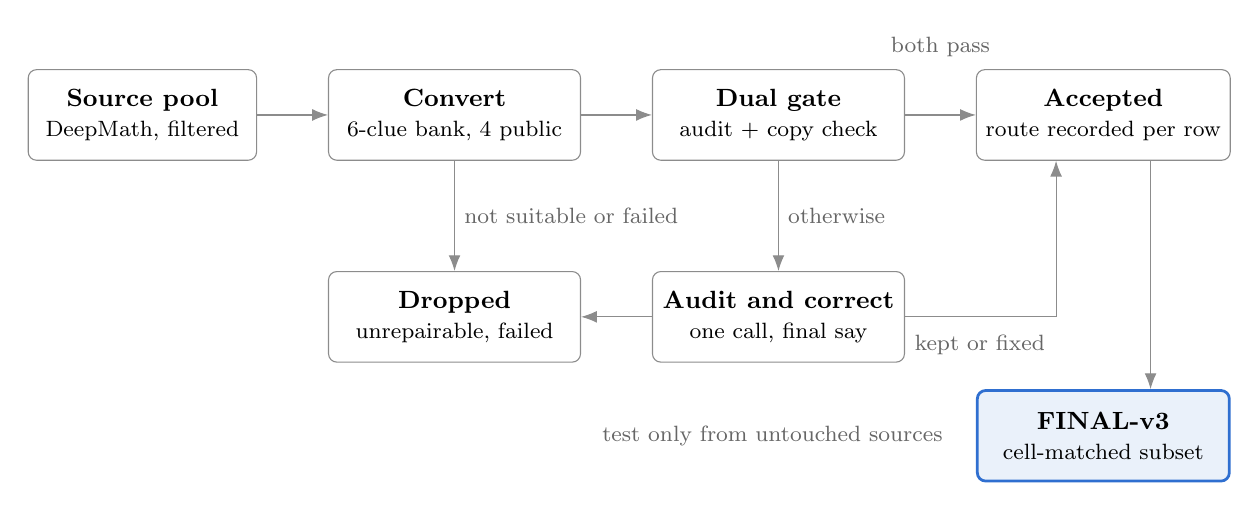
\begin{tikzpicture}[
  box/.style={draw=black!45, rounded corners=3pt, minimum width=3.2cm, minimum height=1.15cm, align=center, font=\small},
  main/.style={box, draw=solve, line width=1pt, fill=solve!10},
  arr/.style={-{Latex[length=2mm]}, draw=black!45},
  lab/.style={font=\footnotesize, text=black!60}]
\node[box, minimum width=2.9cm] (pool) {\textbf{Source pool}\\ \footnotesize DeepMath, filtered};
\node[box, right=0.9cm of pool] (conv) {\textbf{Convert}\\ \footnotesize 6-clue bank, 4 public};
\node[box, right=0.9cm of conv] (gate) {\textbf{Dual gate}\\ \footnotesize audit + copy check};
\node[box, right=0.9cm of gate] (acc) {\textbf{Accepted}\\ \footnotesize route recorded per row};
\node[box, below=1.4cm of gate] (fix) {\textbf{Audit and correct}\\ \footnotesize one call, final say};
\node[box, below=1.4cm of conv] (drop) {\textbf{Dropped}\\ \footnotesize unrepairable, failed};
\node[main, below=2.9cm of acc] (final) {\textbf{FINAL-v3}\\ \footnotesize cell-matched subset};
\draw[arr] (pool) -- (conv);
\draw[arr] (conv) -- (gate);
\draw[arr] (gate) -- (acc);
\node[lab, above=1pt] at ($(gate.north east)!0.5!(acc.north west)$) {both pass};
\draw[arr] (gate) -- node[lab, right] {otherwise} (fix);
\draw[arr] (conv) -- node[lab, right] {not suitable or failed} (drop);
\draw[arr] (fix) -- (drop);
\draw[arr] (fix.east) -| ([xshift=-0.6cm]acc.south);
\node[lab, anchor=north west] at ([yshift=-3pt]fix.east) {kept or fixed};
\draw[arr] ([xshift=0.6cm]acc.south) -- ([xshift=0.6cm]final.north);
\node[lab, left=0.3cm of final] {test only from untouched sources};
\end{tikzpicture}
\caption*{\small Every accepted clue set came through the dual gate or one correction pass; nothing loops back.}
\end{figure}

\paragraph{Step 0 --- the source pool (no API cost).}
\begin{itemize}
\item 380 random 100-row blocks of DeepMath were fetched, and every question already used anywhere in RECONSTRUCT development was excluded first.
\item Shared filters applied; ambiguous multiple-choice answers dropped.
\item Balanced by topic, 1,250 per topic, split 4,000 train / 1,000 test. Difficulty was left at each topic's natural mix, because forcing 8 topic $\times$ band cells to equal size would have capped everything at the scarcest cell (Number Theory upper).
\item The reference solution is DeepMath's first R1 solution, treated as unverified until the audit.
\end{itemize}

\paragraph{Step 1 --- convert} (\code{final\_v1/convert.md}, 16,384 output tokens). The converter sees the question, answer and reference solution and returns either \code{NOT\_SUITABLE} or an ordered bank of \textbf{six} observations, each with a private \code{hidden\_support} note, plus what is withheld and a private certificate showing the original fits. The first four are the public input; the last two are spares. Two few-shot patterns teach the two main moves: hide a premise (a rectangle's area, recovered from the answer) or hide the target (which coefficient is asked for).

\paragraph{Step 2 --- the v1 dual gate} (two independent calls per source).

\begin{table}[H]
\centering\small
\begin{tabularx}{\textwidth}{@{}p{3.2cm}p{3.3cm}L@{}}
\toprule
Check & Sees & Accepts when \\
\midrule
Audit (\code{final\_v1/audit.md}) & source, reference, answer, the 4 clues & answer correct; every clue supported, understandable, distinct; no copy, disguised value or full solution; a named essential element is missing. Leakage quotes must be verbatim public text. \\
Copy challenge (\code{final\_v1/copy.md}) & answer and clues only & it \textbf{cannot} assemble a question using only copy, paraphrase, renaming, reordering and grammar --- no new constraints, targets or inferred premises \\
\bottomrule
\end{tabularx}
\end{table}

A source passes only with audit \code{ACCEPT} \textbf{and} copy \code{no\_direct\_reconstruction}. The copy challenge exists because the audit alone missed near-complete paraphrases: in a 20-source pilot without it, at least 2 of 8 accepted inputs restated the whole question with one parameter dropped.

\paragraph{Step 3 --- audit-and-correct} (\code{runtime/audit\_correct\_p1.md}, added for dataset v1.1). The dual gate accepted only 1,991 of 5,000, far short of the 4,000 needed. Every source it did not accept got \textbf{one} further call that sees the source, reference, the four clues, the two spares and both prior reviews, and returns:
\begin{itemize}
\item \code{ACCEPT\_UNCHANGED} --- the clues were fine;
\item \code{CORRECTED} --- exactly four clues, sound ones kept verbatim, at least one rewritten or swapped for a spare, leaks removed by withholding content (not by rewording it);
\item \code{UNREPAIRABLE} --- wrong answer, ill-posed source, or no coherent four-clue task possible.
\end{itemize}
The prompt was piloted on 40 train-split sources (9 rescued) and then applied unchanged. To limit cost, its decision is final: no second copy challenge, no re-verification.

\begin{table}[H]
\centering\small
\begin{tabular}{@{}llr@{}}
\toprule
Stage & Outcome & Sources \\
\midrule
Convert & not suitable / conversion failed & 15 / 59 \\
v1 dual gate & accepted & \textbf{1,991} \\
 & rejected / unresolved & 2,438 / 497 \\
Audit-and-correct (2,935 eligible) & accepted unchanged & \textbf{751} \\
 & corrected & \textbf{1,275} \\
 & unrepairable / call failed & 486 / 423 \\
\midrule
\textbf{Total accepted} & & \textbf{4,017} \\
\bottomrule
\end{tabular}
\end{table}

\paragraph{Into FINAL-v3.} 4,000 of the 4,017 were kept, matched to the shared cell profile; the 400 test rows come only from the base test pool, which no prompt development (including the corrector pilot) ever touched. The kept rows split by route as 1,981 dual-gate, 1,271 corrected and 748 accepted unchanged, and each row records its route so any subset can be excluded.

\paragraph{Engineering note.} DeepInfra's batch API stalled and let chunks expire, so all stages ran as resumable real-time calls with retries; raw outputs from every round are archived.

\section{RECONSTRUCT: how the design was reached}

The four-clue format was frozen only after about forty small, registered experiments (amendments L through BE in \code{docs/plans/}), each changing one factor on development sources with a local Qwen3-4B student and DeepSeek judges. None of them established a ``best'' version; they established which choices did not help.

\begin{table}[H]
\centering\small
\begin{tabularx}{\textwidth}{@{}p{1.9cm}p{4.6cm}L@{}}
\toprule
Date (2026) & Step & Result \\
\midrule
Sep 28 & FINAL-v3 built & 4,000 of the 4,017 accepted rows kept; training block added \\
Sep 24 & Audit-and-correct added (dataset v1.1) & +2,026 sources accepted; 40-source pilot rescued 9 \\
Sep 23 & Dataset v1 finished & dual gate accepted 1,991 / 5,000 \\
Sep 22 & Copy challenge restored & removing it let near-copies through (pilot BF: $\geq$ 2 of 8) \\
Sep 21 & FINAL\_V1 frozen: four clues + answer & 100-source run: 52 accepted inputs, mean 44.4 / 100, 2 semantic recoveries, 0 fully grounded \\
Sep 20 & Experiments AL--AZ & see lessons below \\
Sep 19--20 & First end-to-end pilot & 1--4 clues; 3 / 8 grounded successes on D1 but 1 / 12 on D2 \\
\bottomrule
\end{tabularx}
\end{table}

\paragraph{What the experiments taught.}
\begin{itemize}
\item \textbf{Fewer clues raise eligibility, not quality.} Three clues let 7 / 16 sources through the gates (mean 28.6) but produced no standalone recovery; four clues became the compromise.
\item \textbf{Loosening the disclosure gate} (AL) raised coverage to 6 / 16 but gave 0 / 6 recoveries.
\item \textbf{Prompt wording barely mattered.} An explicit ``keep the target'' instruction (AM), a changed demonstration (AO) and output order (AJ) showed no reliable gain.
\item \textbf{Reseeding changes nothing.} The same inputs at seeds 0 / 1 / 2 gave identical coarse ratings (AS).
\item \textbf{Richer symbolic clues help most.} Bridge observations plus a premises-first prompt reached 2 verified recoveries in 6 families (AU--AZ), though with a polarised score histogram.
\item \textbf{The judges needed the most work.} The scalar rubric gave full credit to false proofs and graded premises found only in justifications. The partial-credit judges (PC-v1 $\to$ v4) added verbatim-quote certificates and a validator; v4 passes all 19 registered development cases, which fixes tested boundaries but is not proof of general accuracy.
\item \textbf{Direct solving is also a ceiling.} On matched sources, Qwen answered only 7 / 15 SOLVE questions correctly (AQ), so some reconstruction failures are plain mathematics failures.
\end{itemize}

The frozen FINAL\_V1 settings are what the dataset uses: one converter prompt for every source, first four of six clues, dual gate, no per-example tuning, regeneration or filtering by student score.

\section{RECONSTRUCT: intricacies and pitfalls}

\paragraph{Leakage is a mathematical judgment, not a string match.} Ordinary words, needed symbols and shared domain facts are not leaks, and lexical overlap cannot decide the boundary. The subtle cases are values hidden inside true statements. One corrected train row shows this:
\begin{quote}\small
Hidden question: $a_1 = 1$ and $a_{n+1} = (1 + a_1)\cdots(1 + a_n)$; find $\sum_{n \geq 1} 1/(1 + a_n)$. Answer: 1.\\
Original clue 4: \emph{``The recurrence implies $a_{n+1} = a_n(1 + a_n)$.''}\\
Corrected clue 4: \emph{``For $n \geq 2$, the recurrence implies $a_{n+1} = a_n(1 + a_n)$.''}
\end{quote}
The identity holds at $n = 1$ only if $a_1 = 1$, so the original sentence quietly gave away the withheld starting value. Adding ``for $n \geq 2$'' restores a genuine inference: the solver must recover $a_1 = 1$ from the answer.

\paragraph{The corrector certifies its own fixes.} Its decision is final, so nothing independently re-checks the 2,026 rows it accepted. Where a fresh audit plus copy challenge did run on corrected rows (advisory only), 510 passed, 443 were rejected and 322 had no verdict. The 751 rows it accepted \emph{unchanged} had all been rejected or left unresolved by the dual gate. In the pilot, one rescued row gained a solution hint (``examine the expression modulo 3'') that a fresh audit still accepted.

\paragraph{The dual gate is not leak-proof either.} Review of the 100-source FINAL\_V1 run found false copying allegations and one invalid source question that the source-aware audit accepted. No accepted row has had a human audit.

\paragraph{Several questions can fit.} Sparse clues are meant to leave room for sound alternatives, so a correct answer to a \emph{different} well-posed question earns quality credit but not recovery credit. Even the 27B teacher recovers the original question on only 28\% of test items (5\% for the 2B student).

\paragraph{Judging is noisy.} On the test baselines, 62--65 of 400 RECONSTRUCT judgments per model fail certificate validation and stay unresolved. On 100 saved Qwen3-4B responses, a second judge agrees with DeepSeek at Pearson 0.77 on the 0--100 total but only 53\% on the 1--5 rating, so RECONSTRUCT scores are the least reliable of the three tasks.

\paragraph{The training target can mislead.} The training block's \code{final\_answer} is the original question, and its chain of thought (the R1 solution of the original problem) usually restates that question in its first line. Imitating it rewards guessing the source rather than building a question the clues support, so trained models must be evaluated with the source-blind validity judge as well as source recovery. (The OPD study used only \code{training.input}.)

\paragraph{Smaller details.}
\begin{itemize}
\item Deduplication is exact after normalisation; paraphrased duplicates are not detected.
\item Reference solutions are unverified R1 outputs; the audit checks the answer itself and treats the solution as fallible.
\item Whether a question may depend on context outside itself is still an open boundary, reported separately in development runs.
\end{itemize}

\section{Verification and provenance}

\textbf{One script checks all 12,000 rows} against DeepMath-103K and the dataset's own rules: \nolinkurl{.venv/bin/python scripts/audit_final_dataset.py}, which exits non-zero on any failure and prints \code{PROBLEMS: none} (re-run 2 October 2026). It needs only \code{final-v3/} and the DeepMath parquet files.

\begin{table}[H]
\centering\small
\begin{tabularx}{\textwidth}{@{}p{2.6cm}L@{}}
\toprule
Area & What is checked \\
\midrule
Every row & ids (\code{uid} = task + DeepMath row), question hash, question, topic, difficulty, answer and all three reference solutions match DeepMath; no duplicate row or question \\
JUDGE & steps numbered S1..Sn, no five-step items; label, error annotation and teacher target agree; correct items carry no error; the input never contains the key \\
RECONSTRUCT & exactly four non-empty clues; public answer = row answer; neither the input nor any clue contains the source question; acceptance route valid and correction records present exactly when corrected \\
Across tasks & no question shared by two tasks, counting every DeepMath copy \\
Splits & exactly 3,600 / 400, no train--test overlap, test proportional to topic $\times$ difficulty within 0.5 points \\
Rules & JUDGE 2,000 / 2,000 labels, test 200 / 200 and only from the teammate's test split; SOLVE shares = the JUDGE / RECONSTRUCT average; summary counts match \\
\bottomrule
\end{tabularx}
\end{table}

\textbf{Two rules were verified once and cannot be re-checked now}, because they need files that were deleted when old versions were removed: RECONSTRUCT test comes only from untouched sources, and SOLVE excludes every question ever assigned to JUDGE or RECONSTRUCT.

\paragraph{Provenance.} Selection is \nolinkurl{scripts/build_final_datasets_v2.py}, the training block \nolinkurl{scripts/build_final_datasets_v3.py}; both record their own SHA-256 in \code{summary.json}. They read intermediate versions that no longer exist, so they document the method but cannot be re-run end to end. Raw API outputs for every RECONSTRUCT round, clue banks, gate evidence and per-source outcomes are archived in the git-ignored \nolinkurl{local/archive/legacy/reconstruct-dataset-v1-build/}; the teammate's JUDGE files are in \nolinkurl{local/archive/legacy/judge_data/}.

\paragraph{Storage.} The files are gzipped JSONL (\code{\{solve,judge,reconstruct\}-\{train,test\}.jsonl.gz}) because the raw train files (200--265 MB) exceed GitHub's 100 MB limit; \code{CHECKSUMS.txt} lists both forms.

\section{Composition and row schema}

The three tasks line up closely on difficulty and roughly on topic; JUDGE is the least even.

\begin{table}[H]
\centering\small
\begin{tabular}{@{}lrrr@{}}
\toprule
Topic (train / test) & SOLVE & JUDGE & RECONSTRUCT \\
\midrule
Algebra & 893 / 99 & 870 / 97 & 919 / 101 \\
Calculus & 908 / 101 & 899 / 99 & 922 / 102 \\
Discrete Mathematics & 844 / 94 & 820 / 91 & 865 / 97 \\
Number Theory & 955 / 106 & 1,011 / 113 & 894 / 100 \\
\bottomrule
\end{tabular}
\end{table}

\begin{figure}[H]
\centering
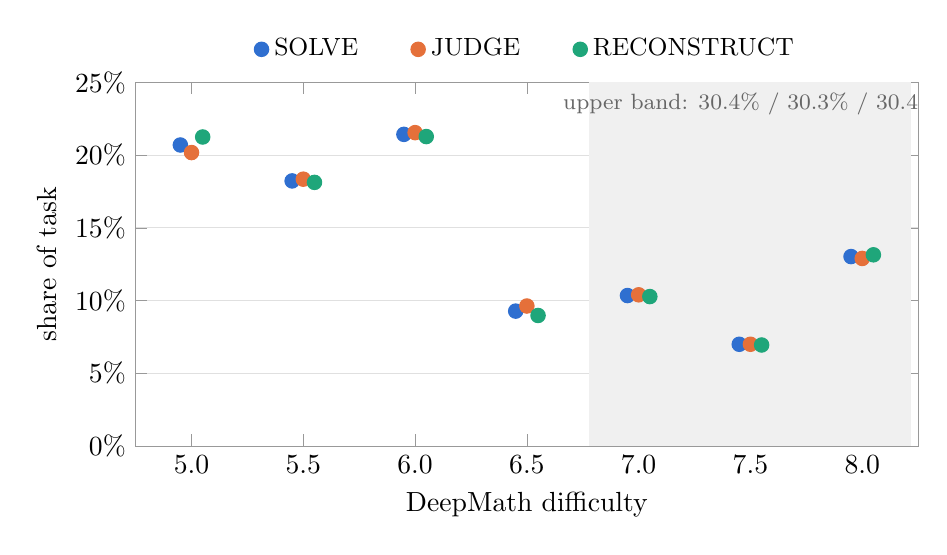
\begin{tikzpicture}
\begin{axis}[
  width=0.95\textwidth, height=6.2cm,
  ymin=0, ymax=25, ytick={0,5,10,15,20,25}, yticklabel={\pgfmathprintnumber{\tick}\%},
  xmin=4.75, xmax=8.25, xtick={5,5.5,6,6.5,7,7.5,8},
  xticklabel style={/pgf/number format/.cd,fixed,fixed zerofill,precision=1},
  xlabel={DeepMath difficulty}, ylabel={share of task},
  ymajorgrids, grid style={black!12}, axis line style={black!40}, tick style={black!40},
  legend style={at={(0.5,1.03)}, anchor=south, legend columns=3, draw=none, font=\small, /tikz/every even column/.append style={column sep=0.6cm}},
  title style={font=\small\bfseries},
  every axis plot/.append style={only marks, mark=*, mark size=2.6pt}]
\fill[black!6] (axis cs:6.78,0) rectangle (axis cs:8.22,25);
\node[font=\footnotesize, text=black!60] at (axis cs:7.5,23.5) {upper band: 30.4\% / 30.3\% / 30.4\%};
\addplot[solve] coordinates {(4.95,20.70) (5.45,18.23) (5.95,21.43) (6.45,9.28) (6.95,10.35) (7.45,7.00) (7.95,13.03)};
\addplot[judge] coordinates {(5.0,20.18) (5.5,18.35) (6.0,21.55) (6.5,9.63) (7.0,10.40) (7.5,7.00) (8.0,12.90)};
\addplot[recon] coordinates {(5.05,21.25) (5.55,18.13) (6.05,21.28) (6.55,8.98) (7.05,10.28) (7.55,6.95) (8.05,13.15)};
\legend{SOLVE, JUDGE, RECONSTRUCT}
\end{axis}
\end{tikzpicture}
\caption*{\small Difficulty shares match across the three tasks within about one point (largest gap: difficulty 5.0, 20.2\% for JUDGE vs 21.3\% for RECONSTRUCT). Source: FINAL-v3 \code{summary.json}, 4,000 questions per task, train + test; upper-band shares in task order.}
\end{figure}

\begin{sloppypar}\paragraph{Fields shared by every row.} \code{task}, \code{split}, \code{uid} (\code{<task>-<DeepMath row>}), \code{dataset\_row\_index}, \code{source\_group\_id} (16-hex hash of the normalised question, the dedup key), \code{topic}, \code{broad\_topic}, \code{difficulty}, \code{difficulty\_band} (lower 5.0--6.5, upper 7.0--8.0), \code{question}, \code{final\_answer}, \code{answer\_normalization}, \code{reference\_solutions} (three R1 solutions), \code{source}, \code{training}.
\end{sloppypar}

\begin{table}[H]
\centering\small
\begin{tabularx}{\textwidth}{@{}p{2.6cm}L@{}}
\toprule
Task & Task-specific fields \\
\midrule
JUDGE & \code{steps}, \code{label}, \code{error\_position}; \code{public} (problem, S1..Sn, instruction); \code{private} (label, first error step, explanation, error type, position, teacher target); \code{friend} (assignment id, original split, provenance hash) \\
RECONSTRUCT & \code{public\_input} (answer + 4 clues); \code{accepted\_by} (route); \code{v1\_status}; \code{audit\_correct} (decision, per-clue findings, reason); \code{original\_public\_input} and \code{corrected\_hidden\_support} on corrected rows; \code{advisory\_fresh\_check} on some corrected rows (not used for acceptance) \\
\bottomrule
\end{tabularx}
\end{table}

\begin{table}[H]
\centering\small
\begin{tabularx}{\textwidth}{@{}lLLL@{}}
\toprule
Task & \code{training.input} & \code{chain\_of\_thought} & \code{final\_answer} \\
\midrule
SOLVE & the question & R1 solution 1 & the answer \\
JUDGE & problem + numbered solution + instruction & none (null) & teacher response \\
RECONSTRUCT & answer + the 4 numbered clues & R1 solution 1 of the original problem & the original question \\
\bottomrule
\end{tabularx}
\end{table}

\section{Limitations}

\begin{enumerate}
\item \textbf{No human audit of RECONSTRUCT inputs.} All 4,000 rows rest on DeepSeek decisions; about half (2,019) were accepted by the corrector without independent re-checking.
\item \textbf{Different questions per task} rule out item-level comparisons, and topic shares differ by up to about three points (JUDGE has the most Number Theory).
\item \textbf{JUDGE's test set is 79\% six-step} while train is 62\%, inherited from the teammate's split.
\item \textbf{Reference solutions are unverified} DeepSeek-R1 outputs; SOLVE and RECONSTRUCT training blocks reuse them as chains of thought.
\item \textbf{Deduplication is exact} after normalisation, so near-paraphrases may still cross tasks or splits.
\item \textbf{The build cannot be re-run end to end}, because intermediate versions were deleted; the audit script verifies the result, not the path to it.
\item \textbf{RECONSTRUCT measurement is noisy}: about 16\% of judgments are unresolved and judge agreement on 1--5 ratings is 53\%.
\item \textbf{No development split} was built into FINAL-v3; later work carved 200 dev questions out of each train split.
\end{enumerate}

\end{document}
